\documentclass[a4paper]{article}
\usepackage{graphicx}
\usepackage[utf8]{inputenc}
\usepackage[english, serbian]{babel}

\title{UseCase: Promena ličnih podataka}
\date{12.11.2018.}

\begin{document}

\maketitle

\begin{itemize}
    \item Akter: Korisnik sistema (Administrator, Glavni urednik, Urednik, Recenzent, Autor)
    \item Kratak opis: Korisnik želi da promeni neke od ličnih podataka
    \item Osnovni tok događaja:
        \begin{enumerate}
            \item Korisniku se prikazuje forma slična onoj koja je korišćena za registraciju, bez pojedinih polja ReCaptcha na kojoj korisnik menja željene podatke.
            \item Korisnik pokušava da promeni podatke.
            \item Novi podaci korisnika su sačuvani.
            \item Nakon uspešne promene podataka sistem obaveštava korisnika o uspešnoj akciji.
        \end{enumerate}
    \item Alternativni tok događaja:
        \begin{enumerate}
            \item Medju promenjenim podacima je i email adresa
                \begin{enumerate}
                    \item Nakon 2. koraka sistem ispisuje poruku uspešnosti promene svih korisničkih podataka osim email adrese. Ispisuje se obaveštenje da korisnik treba da potvrdi svoju novu email adresu tako što će posetiti link koji mu je na tu adresu poslat.
                    \item Korisnik prelazi na korak 3 glavnog toka podataka.
                \end{enumerate}
            \item Neko od obaveznih polja nije popunjeno ili neko od polja ne odgovara formatu koji je za to polje zadat regularnim izrazom
                \begin{enumerate}
                    \item Nakon 2. koraka sistem ispisuje poruku o grešci i obaveštava korisnika da podaci nisu uspešno izmenjeni.
                    \item Korisnik se vraća na korak 1 glavnog toka.
                \end{enumerate}
        \end{enumerate}
\end{itemize}

\begin{figure}
    \centering
    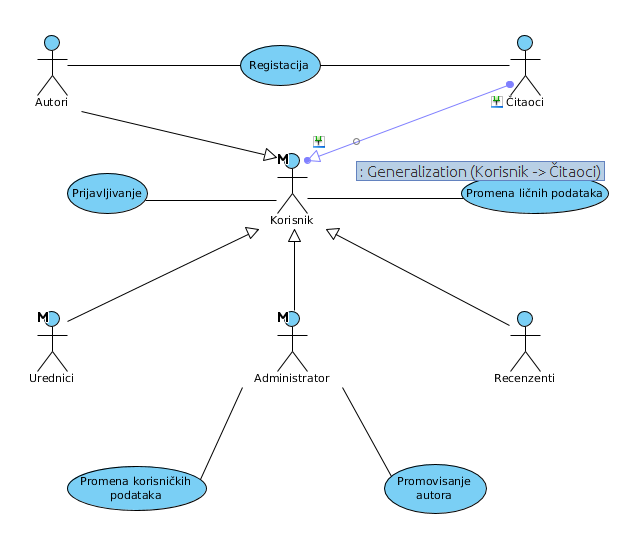
\includegraphics[width=\linewidth]{usecasePrijavljivanje.png}
    \caption{UseCase screenshot}
    \label{fig:my_label}
\end{figure}


\end{document}
